\section{Types of integer programming problems}

In this chapter, we will consider problems in which we have the presence of integer variables. As we will see in the next chapters, the inclusion of integrality requirements imposes further computational and theoretical challenges that we must overcome to be able to solve these problems. On the other hand, being able to consider integer variables allows for the modelling of far more complex and sophisticated systems, to an extent that integer programming problems, or more specifically, mixed-integer programming problems, are by far the most common in practice.

As we did in the first chapter, we will start our discussion by presenting general problems that have particular structures. These structures can often be identified in larger and more complex settings. This will also be helpful in exemplifying how integer variables can be used to model particular features of optimisation problems.

Let us first specify what we mean by an integer programming problem. Our starting point is a linear programming problem:
  %
  \begin{align*}
	  \text{(P)} : \mini \ &c^\top x \\
	  \st & Ax \leq b \\
	  & x \geq 0,
  \end{align*}
  %
  where $A$ is an $m \times n$ matrix, $c$ an $n$-dimensional vector, $b$ an $m$-dimensional vector, and $x$ a vector of $n$ decision variables. 
  
  We say that $P$ is an integer programming problem if the variables $x$ must take integer values, i.e., $x \in \integers^n$. If the variables are further constrained to be binary, i.e., $x \in \braces{0,1}^n$, we say that it is a binary programming problem. Perhaps the most common setting is when only a subset of the variables are constrained to be integer or binary (say $p$ of them), $x \in \reals^{n-p} \times \integers^p$. This is what is referred to as \emph{mixed-integer programming}, or MIP. The most common setting for integer programming problems is to have binary variables only, or a combination of binary and continuous variables. 
   
One important distinction must be made. A closely related concept is that of \emph{combinatorial optimisation problems}, which refer to problems of the form
%
\begin{align*}
 	\mini_{S \subseteq N} \braces{\sum_{j \in S} c_j : S \in \mathcal{F} \subseteq N},
\end{align*}
%
where $c_j$, $j \in N$, is a weight, and $\mathcal{F}$ is a family of feasible subsets. As the name suggests, in these problems we are trying to form combinations of elements such that a measure (i.e., an objective function) is optimised. Integer programming happens to be an important framework for expressing combinatorial optimisation problems, though both integer programming and combinatorial optimisation expand further to other settings as well. To see this connection, let us define an \emph{incidence vector} $x^S$ of $S$ such that
%
  \begin{align*}
	  x^S_j = \begin{cases}
	       1, \text{if } j \in S \\ 
	       0, \text{otherwise}.
	     \end{cases}
  \end{align*}
%
Incidence vectors will permeate many of the (mixed-)integer programming formulations we will see. Notice that, once $x^S$ is defined, the objective function simply becomes $\sum_{j \in N} c_j x_j$. Integer programming formulations are particularly suited for combinatorial optimisation problems when $\mathcal{F}$ can be represented by a collection of linear constraints. 


\section{(Mixed-)integer programming applications}

We will consider now a few examples of integer and mixed-integer programming models with somewhat general structure. As we will see, many of these examples have features that can be combined into more general models.


\subsection{The assignment problem}

Consider the following setting. Assume that we must execute $n$ jobs, which must be assigned to $n$ distinct workers. Each job can be assigned to a worker only, and, analogously, each worker can only be assigned to one job. Assigning a worker $i$ to a job $j$ costs $C_{ij}$, which could measure, e.g., the time taken by worker $i$ to execute job $j$. Our objective is to find a minimum cost assignment between workers and jobs. Figure \ref{p1c8:fig:assignment_a} illustrates all possible worker-job assignments as arcs between nodes representing workers on the left and jobs on the right. Figure \ref{p1c8:fig:assignment_b} represents one possible assignment.
%
\begin{figure}[h]
	\begin{subfigure}[b]{0.49\textwidth}
		\centering
		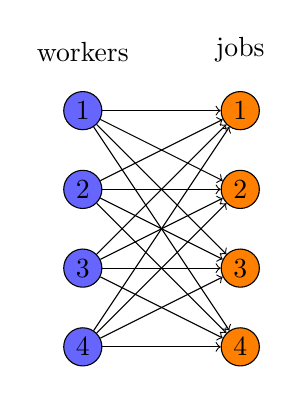
\begin{tikzpicture}[scale=1,
		node/.style={circle, fill=blue!60, draw, minimum size=1em, inner sep=2pt},
		node2/.style={circle, fill=orange, draw, minimum size=1em, inner sep=2pt}] 
		    \node[above] at (0, 3.5) {workers};                                                                                  
		    \node[above] at (2, 3.5) {jobs};
		    \node[node] (1) at (0, 3) {1};
		    \node[node] (2) at (0, 2) {2};
		    \node[node] (3) at (0, 1) {3};
		    \node[node] (4) at (0, 0) {4};
		    \node[node2] (5) at (2, 3) {1};
		    \node[node2] (6) at (2, 2) {2};
		    \node[node2] (7) at (2, 1) {3};
		    \node[node2] (8) at (2, 0) {4};
		  
 		    \foreach \x in {1,...,4} {
 		       \foreach \y in {5,...,8} {
		          \draw[->] (\x) -- (\y);
		          }} 
		\end{tikzpicture}
		\caption{} \label{p1c8:fig:assignment_a}
	\end{subfigure}
	\hfill
	\begin{subfigure}[b]{0.49\textwidth}
		\centering
		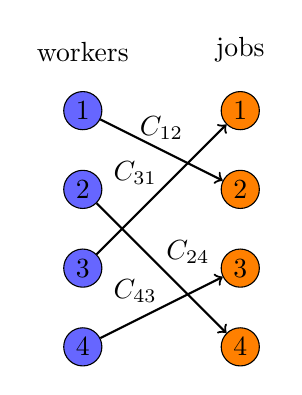
\begin{tikzpicture}[scale=1,
			node/.style={circle, fill=blue!60, draw, minimum size=1em, inner sep=2pt},
			node2/.style={circle, fill=orange, draw, minimum size=1em, inner sep=2pt}] 
			\node[above] at (0, 3.5) {workers};                                                                                  
			\node[above] at (2, 3.5) {jobs};
			\node[node] (1) at (0, 3) {1};
			\node[node] (2) at (0, 2) {2};
			\node[node] (3) at (0, 1) {3};
			\node[node] (4) at (0, 0) {4};
			\node[node2] (5) at (2, 3) {1};
			\node[node2] (6) at (2, 2) {2};
			\node[node2] (7) at (2, 1) {3};
			\node[node2] (8) at (2, 0) {4};
			\draw[->, thick] (1) -- node[above]{$C_{12}$} (6);
		    \draw[->, thick] (2) -- node[above right = -2]{$C_{24}$} (8);
		    \draw[->, thick] (3) -- node[above left = -2]{$C_{31}$} (5);
		    \draw[->, thick] (4) -- node[above left=-2]{$C_{43}$} (7);                                          
		\end{tikzpicture}
		\caption{} \label{p1c8:fig:assignment_b}
	\end{subfigure}
	\caption{An illustration of all potential assignments as a graph and an example of one possible assignment, with total cost $C_{12}$ + $C_{31}$ + $C_{24}$ + $C_{43}$}			
\end{figure}

To represent the problem, let $x_{ij} =$ 1 if worker $i$ is assigned to job $j$ and 0, otherwise. Let $N = \braces{1,\dots,n}$ be a set of indices of workers and jobs (we can use the same set since they are of same number). The integer programming model that represent the assignment problem is given by
%  
\begin{align*} 
  (AP) : \mini \ & \sum_{i \in N}\sum_{j \in N} C_{ij}x_{ij} \\
  \st & \sum_{j \in N} x_{ij} = 1, \ \forall i \in N\\
      & \sum_{i \in N} x_{ij} = 1, \ \forall j \in N\\
      & x_{ij} \in \braces{0,1},  \ \forall i, \forall j \in N.
\end{align*}
%

Before we proceed, let us make a parallel to combinatorial problems. The assignment problem is an example of a combinatorial problem, which can be posed by making (i) $N$ the set of all job-worker pairs $(i,j)$; (ii) $S \in \mathcal{F}$ the $(i,j)$ pairs in which $i$ and $j$ appear in exactly one pair, and, (iii) $x^S$ such that $x_{ij}, i,j = 1,\dots,n$. Thus, the assignment problem is an example of a combinatorial optimisation problem that can be represented as an integer programming formulation.


\subsection{The knapsack problem}

The knapsack problem is another combinatorial optimisation problem that arises in several applications. Consider that we have a collection of $n$ items from which we must make a selection. Each item has associated a cost $A_i$ (e.g., weight) and our selection must be such that the total cost associated with the selection does not exceed a budget $B$ (e.g., weight limit). Each item has also a value $C_i$ associated, and our objective is to find a maximum-valued selection of items such that it does not exceed the budget. 

To model that, let us define $x_{i} =$ 1 if item $i$ is selected and 0, otherwise. Let $N = \braces{1,\dots,n}$ be the set of items. Then, the knapsack problem can be represented as the following integer programming problem     
%  
\begin{align*}
	(KP) : \maxi_x \ & \sum_{i=1}^nC_{i}x_{i} \\
	\st & \sum_{i = 1}^n A_{i}x_{i} \leq B\\
	  & x_{i} \in \braces{0,1}, \ \forall i \in N. 
\end{align*}

Notice that the knapsack problem has variants in which an item can be selected a certain number of times, or that multiple knapsacks must be considered simultaneously, both being generalisations of $KP$. 

Also, the knapsack problem is also a combinatorial optimisation problem, which can be stated by (i) making $N$ the set of all items $\braces{1,\dots, n}$, (ii) $S \in \mathcal{F}$ the subset of items with total cost not greater than $B$, and (iii) $x^S$ such that $x_{i}, \forall i \in N$.   


\subsection{The generalised assignment problem}

The generalised assignment problem (or GAP) is a generalisation of the assignment problem including a structure that resembles that of a knapsack problem. In this case, we consider the notion of bins, to each the items have to be assigned. In this case, multiple items can be assigned to a bin, or a bin might have no item assigned. In some contexts, this problem is also known as the \emph{bin packing problem}. 

In this case, we would like to assign all of the $m$ items to $n$ bins, observing that the capacity $B$ of each bin cannot be exceeded by the weights $A_i$ of the items assigned to that bin. We know that assigning the item $i=1,\dots,m$ to the bin $j=1,\dots,n$ costs $C_{ij}$. Our objective is to obtain a minimum-cost bin assignment (or packing) that does not exceed any of the bin capacities. Figure \ref{p1c8:fig:bin_packing} illustrates a possible assignment of items to bins. Notice that the number of total bins does not necessarily need to be the same the number of items. 

\begin{figure}
	\centering
	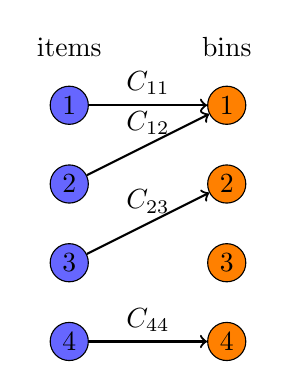
\begin{tikzpicture}[scale=1,
	node/.style={circle, fill=blue!60, draw, minimum size=1em, inner sep=2pt},
	node2/.style={circle, fill=orange, draw, minimum size=1em, inner sep=2pt}] 
	    \node[above] at (0, 3.5) {items};                                                                                  
	    \node[above] at (2, 3.5) {bins};
	    \node[node] (1) at (0, 3) {1};
	    \node[node] (2) at (0, 2) {2};
	    \node[node] (3) at (0, 1) {3};
	    \node[node] (4) at (0, 0) {4};
	    \node[node2] (5) at (2, 3) {1};
	    \node[node2] (6) at (2, 2) {2};
	    \node[node2] (7) at (2, 1) {3};
	    \node[node2] (8) at (2, 0) {4}; 
	    \draw[->, thick] (1) -- node[above]{$C_{11}$} (5);
	    \draw[->, thick] (2) -- node[above]{$C_{12}$} (5);
	    \draw[->, thick] (3) -- node[above]{$C_{23}$} (6);
	    \draw[->, thick] (4) -- node[above]{$C_{44}$} (8);                                           
	\end{tikzpicture}
	\caption	{An example of a bin packing with total cost $C_{11}$ + $C_{12}$ + $C_{23}$ + $C_{44}$} \label{p1c8:fig:bin_packing}
\end{figure}

To formulate the generalised assignment problem as an integer programming problem, let us define $x_{ij} =$ 1, if item $i$ is packed into bin $j$, and $x_{ij} = 0$ otherwise. Moreover, let $M = \braces{1,\dots,m}$ be the set of items and $N = \braces{1,\dots,n}$ be the set of bins. Then, the problem can be formulated as follows.

\begin{align*}
	(GAP) : \mini_x \ & \sum_{i \in M}\sum_{j \in N} C_{ij}x_{ij} \\
	\st & \sum_{j=1}^n x_{ij} = 1, \forall i \in M\\
	  & \sum_{i=1}^m A_{i}x_{ij} \leq B_j, \forall j \in N\\
	  & x_{ij} \in \braces{0,1}, \forall i \in M, \forall j \in N. 
\end{align*} 

Hopefully, the parallel to the combinatorial optimisation problem version is clear at this point and is let for the reader as a thought exercise. 


\subsection{The set covering problem}

Set covering problems are related to the location of infrastructure (or facilities) with the objective of covering demand points and, thus, frequently recurring in settings where service centres such as fire brigades, hospitals, or police stations must be located to efficiently serve locations.

Let $M = \{1,\dots,m\}$ be a set of regions that must be served by opening \emph{service centres}. A centre can be opened at any of the $N = \{1,\dots,n\}$ possible locations. If a centre is opened at location $J \in N$, then it serves (or covers) a subset of regions $S_j \subseteq M$ and has associated opening cost $C_j$. Our objective is to decide where to open the centres so that all regions are served and the total opening cost is minimised. 

Figure \ref{p1c8:fig:set_covering} illustrates an example of a set covering problem based on a fictitious map broken into regions. Each of the cells represents a region that must be covered, i.e., $M = \braces{1,\dots, 20}$. The blue cells represent regions that can have a centre opened, that is, $N = \braces{3,4,7,11,12,14,19}$. Notice that $N \subset M$. In this case, we assume that if a centre is opened at a blue cell, then it can serve the respective cell and all adjacent cells. Therefore, we have, e.g., that $S_3 = \braces{1,2,3,8}$, $S_4=\braces{2,4,5,6,7}$, and so forth.

\begin{figure}[h]
	\centering
	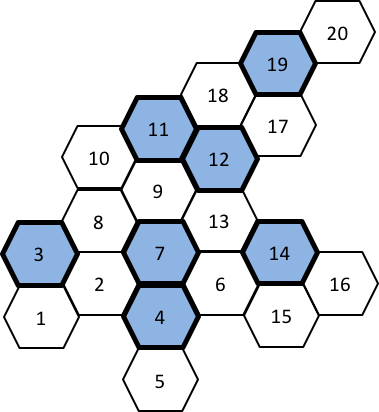
\includegraphics[scale=0.8]{part_1/chapter_8/figures/hive_setcover.png}
	\caption{The hive map illustrating the set covering problem. Our objective is to cover all of the regions while minimising the total cost incurred by opening the centres at the blue cells} \label{p1c8:fig:set_covering}
\end{figure}

To model the set covering problem, and pretty much any other problem involving indexed subsets such as $S_j$, $\forall j \in N$, we need an auxiliary parameter matrix $A$, often referred to as \emph{0-1 incidence matrix} such that
%
\begin{equation*}
	A = \begin{cases}
		A_{ij} = 1, \text{ if } i \in S_j, \\
		A_{ij} = 0, \text{ otherwise.}
	\end{cases}
\end{equation*}
%
For example, referring to Figure \ref{p1c8:fig:set_covering}, the first column of $A$ would refer to $j = 3$ and would have nonzero values at rows 1, 2, 3, and 8.

We are now ready to pose the set covering problem as an integer programming problem. For that, let $x_{j} = 1$ if a facility is opened (or a service centre is located) at location $j$ and $x_j = 0$, otherwise. In addition, let $M = \braces{1,\dots,m}$ be the set of regions to be served and $N = \braces{1,\dots,n}$ be the set of candidate places to have a facility opened. Then, the set covering problem can be formulated as follows.
%
\begin{align*}
  (SCP) : \mini_x \ & \sum_{j \in N} C_{j}x_{j} \\
  \st & \sum_{j \in N} A_{ij}x_{j} \geq 1, \forall i \in M\\
      & x_{j} \in \braces{0,1}, \forall j \in N. 
\end{align*}
%
As a final note, notice that this problem can also be posed as a combinatorial optimisation problem of the form
%
\begin{align*}
  \mini_{T \subseteq N} \braces{\sum_{j \in T} C_j : \bigcup_{j \in T}S_j = M},
\end{align*}
%
in which the locations $j \in T$ can be represented as an incidence vector, as before.


\subsection{Travelling salesperson problem}

The travelling salesperson problem (TSP) is one of the most famous combinatorial optimisation problems, perhaps due to its interesting mix of simplicity while being computationally challenging. Assume that we must visit a collection of $n$ cities at most once, and return to our initial point, forming a so-called \emph{tour}. When travelling from a city $i$ to a city $j$, we incur in the cost $C_{ij}$, representing, for example, distance or time. Our objective is to minimise the total cost of our tour. Notice that this is equivalent to finding the minimal cost permutation of $n-1$ cities, discarding the city which represents our starting and end point. Figure \ref{p1c8:fig:TSP} illustrates a collection of cities and one possible tour.

\begin{figure}[h]
	\centering
	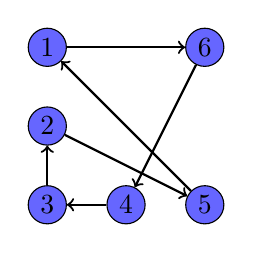
\begin{tikzpicture}[node/.style={circle, fill=blue!60, draw, minimum size=1em, inner sep=2pt}, scale=1]
	    \node[node] (3) at (0, 0)  {3};
	    \node[node] (2) at (0, 1)  {2};
	    \node[node] (4) at (1, 0)  {4};
	    \node[node] (5) at (2, 0)  {5};
	    \node[node] (1) at (0, 2)  {1};
	    \node[node] (6) at (2, 2)  {6};     
	    \draw[->, thick] (1) -- (6);
	    \draw[->, thick] (6) -- (4);
	    \draw[->, thick] (4) -- (3);
	    \draw[->, thick] (3) -- (2);
	    \draw[->, thick] (2) -- (5);
	    \draw[->, thick] (5) -- (1);
	\end{tikzpicture}
	\caption{An example of a tour between the six cities} \label{p1c8:fig:TSP}
\end{figure}

To pose the problem as an integer programming model, let us define $x_{ij} =$ 1 if city $j$ is visited directly after city $i$, and $x_{ij} = 0$ otherwise. Let $N = \braces{1,\dots,n}$ be the set of cities. We assume that $x_{ii}$ is not defined for $i \in N$. A naive model for the travelling salesperson problem would be 
%
\begin{flalign*}
	(TSP) : \mini_x \ & \sum_{i \in N}\sum_{j \in N}C_{ij}x_{ij} \\
	\st & \sum_{j \in N \setminus \braces{i}} x_{ij} = 1, \forall i \in N\\
	& \sum_{i \in N \setminus \braces{j}} x_{ij} = 1, \forall j \in N\\
	& x_{ij} \in \braces{0,1}, \forall i,\forall j \in N : i \neq j
\end{flalign*}
%
First, notice that the formulation of $TSP$ is exactly the same as that of the assignment problem. However, this formulation has an issue. Although it can guarantee that all cities are only visited once, it cannot enforce an important feature of the problem which is that the tour cannot present disconnections, i.e., contain \emph{sub-tours}. In other words, the salesperson must physically visit from city to city in the tour, and cannot ``tele-transport'' from one city to another. Figure \ref{p1c8:fig:TSP_subtours} illustrates the concept of sub-tours.

\begin{figure}[h]
	\centering	
	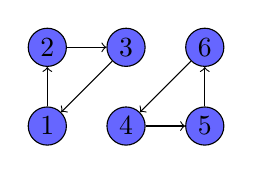
\begin{tikzpicture}[node/.style={circle, fill=blue!60, draw, minimum size=1em, inner sep=2pt}]
		\node[node] (1) at (0, 0) {1};
		\node[node] (2) at (0, 1) {2};
		\node[node] (3) at (1, 1) {3};
		\node[node] (4) at (1, 0) {4};
		\node[node] (5) at (2, 0) {5};
		\node[node] (6) at (2, 1) {6};			
		\draw[->] (1) -- (2);
		\draw[->] (2) -- (3);
		\draw[->] (3) -- (1);
		\draw[->] (4) -- (5);
		\draw[->] (5) -- (6);
		\draw[->] (6) -- (4);
	\end{tikzpicture}
	\caption{A feasible solution for the naive TSP model. Notice the two sub-tours formed} \label{p1c8:fig:TSP_subtours}
\end{figure}

In order to prevent sub-tours, we must include constraints that can enforce the full connectivity of the tour. There are mainly two types of such constraints. The first is called \emph{cut-set constraints} and is defined as
%
\begin{equation*} 
	\sum_{i \in S}\sum_{j \in N \setminus S}x_{ij} \geq 1, \forall S \subset N, 2 \leq |S| \leq n-1. 
\end{equation*}
%
The cut-set constraints act by guaranteeing that among any subset of nodes $S \subseteq N$ there is always at least one arc $(i,j)$ connecting one of the nodes in $S$ and a node not in $S$. 

An alternative type of constraint is called \emph{sub-tour elimination} constraint and is of the form
%
\begin{equation*}
	\sum_{i \in S}\sum_{j \in S}x_{ij} \leq |S|-1, \forall S \subset N, 2 \leq |S| \leq n-1. 
\end{equation*}
%
Differently from the cutset constraints, the sub-tour elimination constraints prevent the cardinality of the nodes in each subset to match the cardinality of arcs within the same subset.

For example, consider the sub-tours illustrated in Figure \ref{p1c8:fig:TSP_subtours} and assume that we would like to prevent the sub-tour formed by $S = \braces{1,2,3}$. Then the cutset constraint would be of the form

\begin{equation*}
	x_{14} + x_{24} + x_{34} + x_{15} + x_{25} + x_{35} + x_{16} + x_{26} + x_{36}\geq 1	
\end{equation*}
%
while the sub-tour elimination would be of the form
\begin{equation*}
	x_{12} + x_{13} + x_{21} + x_{23} + x_{31} + x_{32} \leq 2
\end{equation*}
%
There are some differences between these two constraints and, typically cutset, constraints are preferred for being stronger (we will discuss the notion of stronger constraints in the next chapters). In any case, either of them suffers from the same problem: the number of such constraints quickly becomes computationally prohibitive as the number of nodes increases. This is because one would have to generate a constraint to each possible node subset combination from sizes 2 to $n-1$. 

A possible remedy to this consists of relying on delayed constraint generation. In this case, one can start from the naive formulation $TSP$ and from the solution, observe whether there are any sub-tours formed. That being the case, only the constraints eliminating the observed sub-tours need to be generated, and the problem can be warm-started. This procedure typically terminates far earlier than having all of the possible cutset or sub-tour elimination constraints generated. 


\subsection{Uncapacitated facility location}

This is the first mixed-integer programming we consider. In this, we would like to design a network that can supply clients $i \in M$ by opening (or locating, as it is referred to in this context) facilities among candidate locations $j \in N$. Opening a facility incurs in the fixed cost $F_j$, and serving a client $i \in M$ from a facility that has been located at $j \in N$ costs $C_{ij}$. Our objective is to design the most cost-effective production and distribution network. That is, we must decide where to locate facilities and how to serve clients (from these facilities) with minimum total (locating plus service) cost. Figure \ref{p1c8:fig:facility_location_a} illustrates an example of the problem with $M = \braces{1,\dots,8}$ and $N = \braces{1,\dots,6}$ and Figure \ref{p1c8:fig:facility_location_b} presents one possible configuration with two facilities. The optimal number of facilities located and the client-facility association depends on the trade-offs between locating and service costs.	

\begin{figure}[h]
	\begin{subfigure}[b]{0.49\textwidth}
		\centering 
		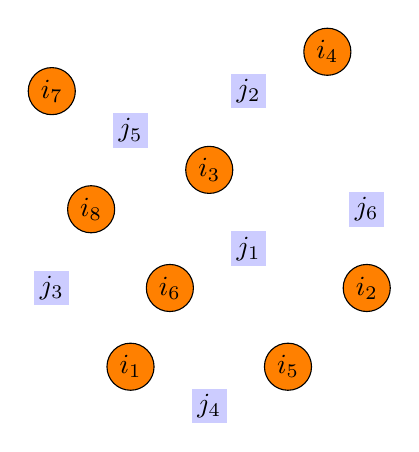
\begin{tikzpicture}[scale = 0.5, 
	      	client/.style={circle, draw, fill=orange, minimum size=1em, inner sep=2pt},
	      	depot/.style={fill=blue!20, minimum size=1em, inner sep=2pt},
	      	located/.style={draw, fill=blue, minimum size=1em, inner sep=2pt}]
	          \node[client] (1) at (3,2) {$i_1$};
	          \node[client] (2) at (9,4) {$i_2$};
	          \node[client] (3) at (5,7) {$i_3$};
	          \node[client] (4) at (8,10) {$i_4$};
	          \node[client] (5) at (7,2) {$i_5$};
	          \node[client] (6) at (4,4) {$i_6$};
	          \node[client] (7) at (1,9) {$i_7$};
	          \node[client] (8) at (2,6) {$i_8$};
	          \node[depot]  (9) at (6,5) {$j_1$};
	          \node[depot] (10) at (6,9) {$j_2$};
	          \node[depot] (11) at (1,4) {$j_3$};
	          \node[depot] (12) at (5,1) {$j_4$};
	          \node[depot] (13) at (3,8) {$j_5$};
	          \node[depot] (14) at (9,6) {$j_6$};
	      \end{tikzpicture}
	      \caption{} \label{p1c8:fig:facility_location_a}	
	\end{subfigure}
	\hfill
	\begin{subfigure}[b]{0.49\textwidth}
		\centering
		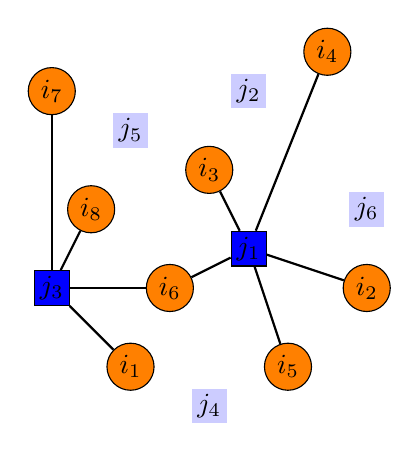
\begin{tikzpicture}[scale = 0.5, 
	      	client/.style={circle, draw, fill=orange, minimum size=1em, inner sep=2pt},
	      	depot/.style={fill=blue!20, minimum size=1em, inner sep=2pt},
	      	located/.style={draw, fill=blue, minimum size=1em, inner sep=2pt}]
	          \node[client] (1) at (3,2) {$i_1$};
	          \node[client] (2) at (9,4) {$i_2$};
	          \node[client] (3) at (5,7) {$i_3$};
	          \node[client] (4) at (8,10) {$i_4$};
	          \node[client] (5) at (7,2) {$i_5$};
	          \node[client] (6) at (4,4) {$i_6$};
	          \node[client] (7) at (1,9) {$i_7$};
	          \node[client] (8) at (2,6) {$i_8$};
	          \node[depot]  (9) at (6,5) {$j_1$};
	          \node[depot] (10) at (6,9) {$j_2$};
	          \node[depot] (11) at (1,4) {$j_3$};
	          \node[depot] (12) at (5,1) {$j_4$};
	          \node[depot] (13) at (3,8) {$j_5$};
	          \node[depot] (14) at (9,6) {$j_6$};
	          \node[located] (11) at (1,4) {$j_3$};
	          \node[located] (9) at (6,5) {$j_1$};
	          \draw[-, thick] (4) -- (9);
	          \draw[-, thick] (3) -- (9);
	          \draw[-, thick] (2) -- (9);
	          \draw[-, thick] (5) -- (9);
	          \draw[-, thick] (6) -- (9);
	          \draw[-, thick] (8) -- (11);
	          \draw[-, thick] (6) -- (11);
	          \draw[-, thick] (1) -- (11);
	          \draw[-, thick] (7) -- (11);
	      \end{tikzpicture}
	      \caption{}\label{p1c8:fig:facility_location_b}
	\end{subfigure}
	\caption{An illustration of the facility location problem and one possible solution with two facilities located (right)}	
\end{figure}
 
To formulate the problem as a mixed-integer programming problem, let us define $x_{ij}$ as the fraction of the demand in $i \in M$ being served by a facility located at $j \in N$. In addition, we define the binary variable $y_j$ such that $y_j = 1$, if a facility is located at $j \in N$ and 0, otherwise. With those, the uncapacitated facility location (or UFL) problem can be formulated as 
%
\begin{flalign}
	(UFL) : \mini_{x,y} \ & \sum_{j \in N} F_jy_j +  \sum_{i \in M}\sum_{j \in N} C_{ij}x_{ij} \\
	\st & \sum_{j \in N} x_{ij} = 1, \forall i \in M\\
	& \sum_{i \in M} x_{ij} \leq m y_j, \forall j \in N \label{p1c8:eq:big-M_UFL}\\
	&x_{ij} \geq 0, \forall i \in M, \forall j \in N\\
	&y_j \in \braces{0,1}, \forall j \in N.
\end{flalign}

Some features of this model are worth highlighting. First, notice that the absolute values associated with the demand at nodes $i \in M$ are somewhat implicitly represented in the cost parameter $C_{ij}$. This is an important modelling feature that allows the formulation to be not only stronger but also more numerically favourable (avoiding large coefficients). Therefore, the demand is thought as being, at each node, 1 or 100\%, and $0 \le x_{ij} \le 1$ represents the fraction of the demand at $i \in M$ being served by a facility eventually located at $j \in N$. Second, notice how the variable $x_{ij}$ is only allowed to be greater than zero if the variable $y_j$ is set to 1, due to \eqref{p1c8:eq:big-M_UFL}. Notice that $m$, the number of clients, is acting as a maximum upper bound for the amount of demand being served from the facility $j$, which would be at most $m$ when only one facility is located. That constraint is precisely the reason why the problem is called uncapacitated, since, in principle, there are no capacity limitations on how much demand is served from a facility. 

Facility location problems are frequent in applications associated with supply chain planning problems and can be specialised to a multitude of settings, including capacitated versions (both nodes and arcs), versions where the arcs must also be located (or built), having multiple echelons, and so forth. 

 
\subsection{Uncapacitated lot-sizing}

Another example of an important mixed-integer programming formulation is the uncapacitated lot-sizing. In this, we would like to plan the production of a single product over a collection of time periods $T = \braces{1, \dots, n}$. We have encountered this problem before in Chapter \ref{chapter_1}, but now we consider the variation in which the production activity implies in a fixed cost $F_t$, representing, for example, a setup cost or the need for renting equipment. Once again, we incur a cost $C_t$ to produce one unit in period $t$ and $H_t$ is paid to store one unit of product from period $t$ to period $t+1$.

Let us define $p_t \geq 0$ be the amount produced in period $t\in T$, and $s_t \geq 0$ as the amount stored at the end of period $t \in T$. In addition, let $y_t \in \braces{0,1}$ indicate whether production occurs in period $t\in T$. Also, assume that $M$ is a sufficiently large constraint. Then, the uncapacitated lot-sizing (ULS) can be formulated as
%
\begin{align}
	(ULS) : \mini_{x,s,y} \ & \sum_{t \in N} (F_ty_t + P_tp_t + H_ts_t) \nonumber \\
	\st & s_{t-1} + p_t = d_t + s_t, \forall t \in N \nonumber \\
	& p_t \leq My_t, \forall t \in N  \label{p1c8:eq:big_M_ULS}\\
	&s_t, p_t \geq 0, \forall t \in N \nonumber \\
	&y_t \in \braces{0,1}, \forall t \in N. \nonumber
\end{align} 

Notice that the formulation of $ULS$ is very similar to that seen in Chapter \ref{chapter_1}, with exception of the variable $y_t$, its associated fixed cost term $\sum_{t \in T} F_jy_j$ and the constraint \eqref{p1c8:eq:big_M_ULS}. This constraint is precisely what renders the ``uncapacitated'' nomenclature, and is commonly known in the context of mixed-integer programming as \emph{big-M constraints}. Notice that the constant $M$ is playing the role of $+\infty$: it only really makes the constraint relevant when $y_t = 0$, so that $p_t \le 0$ is enforced, making thus $p_t = 0$. However, this interpretation has to be taken carefully. Big-M constraints are known for being the cause of numerical issues and worsening the performance of mixed-integer programming solver methods. Thus, the value of $M$ must be set such that it is the smallest value possible such that it does not artificially create a constraint. Finding these values are often challenging and instance dependent. In the capacitated case, $M$ can trivially take the value of the production capacity. 
 
  
\section{Good formulations}

In this section, we discuss what makes a formulation a better formulation for a (mixed-)integer programming (MIP) problem. Just like it is the case with any mathematical programming application, there are potentially infinite possible ways to formulate the same problem. While in the case of linear programming (i.e., only continuous variables), alternative formulations typically do not lead to significant differences in terms of computational performance, the same is definitely not true in the context of MIP. In fact, whether a MIP problem can be solved in a reasonable computational time often depend on having a good, or \emph{strong}, formulation.

Therefore, it is fundamental that we can recognise which of alternative formulations might yield better computational performance. But first, we must be able to understand the source of these differences. For that, the first thing to realise is that solution methods for MIP models rely on \emph{successively solving linear programming models} called \emph{linear programming (LP) relaxations}. How exactly this happens will be the subject of our next chapters. But for now, one can infer that the best formulation will be the one that requires the solution of the least of such LP relaxations. And precisely, it so turns out that the number of LP relaxations that need to be solved (and, hence, performance) is strongly dependent on how closely it resembles the \emph{convex hull} of the feasible solutions.

An LP relaxation simply consists of a version of the original MIP problem in which the integrality requirements are dropped. Most of the methods used to solve MIP models are based on LP relaxation. There are several reasons why the employment of LP relaxations is a good strategy. First, we can solve (and resolve) LP problems efficiently. Secondly, the solution of the LP relaxation can be used to \emph{reduce} the search space of the original MIP. However, simply rounding the solution of the LP relaxation will typically not lead to relevant solutions.

Let us illustrate the geometry of an integer programming model, such that the points we were discussing become more evident. Consider the problem
%
\begin{align*}
	(P): \maxi_x &x_1 + \frac{16}{25}x_2 \\
	\st &50x_1 + 31x_2 \leq 250\\
	&3x_1 + 31x_2 \geq -4\\
	&x_1, x_2 \in \integers_+.
\end{align*}
 
The feasible region of problem $P$ is represented in Figure \ref{p1c8:fig:IP_feasible_region}. First, notice how in this case the feasible region is not a polyhedral set anymore, but yet a collection of discrete points (represented in blue) that happen to be within the polyhedral set formed the linear constraints. This is one of the main complicating features of MIPs because the premise of convexity does not hold anymore. Another point can be noticed in Figure \ref{p1c8:fig:IP_feasible_region}. Notice that rounding the solution obtained from the LP relaxation would in most cases lead to infeasible solutions, except when $x_1$ is rounded up and $x_2$ rounded down, which leads to the suboptimal solution $(2,5)$. However, one can still graphically find the optimal solution using exactly the same procedure as that employed for linear programming problems, which would lead to the optimal integer solution $(5,0)$.

\begin{figure}[h]
	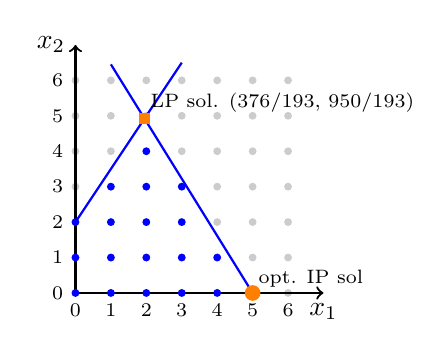
\begin{tikzpicture}[scale = 0.45,
		  point/.style={circle, fill=gray!40, inner sep=1pt},
		  feas point/.style={circle, fill=blue, inner sep=1pt}]
		  \foreach \x in {0,...,6}{
		      \foreach \y in {0,...,6} {
		          \node[point] (\x,\y) at (\x, \y) {};
		      }}
		  \foreach \x in {0,...,6}{
		      \node[font=\scriptsize] at (\x,-0.5) {$\x$};
		  }
		  \foreach \y in {0,...,6}{
		      \node[font=\scriptsize] at (-0.5,\y) {$\y$};
		  }                      
		  \draw[thick, <->] (7,0) node[below]{$x_1$} -- (0,0) -- (0,7) node[left]{$x_2$};  
		  \draw[domain=1:5, thick,variable=\x,blue] plot ({\x},{250/31 - 50/31*\x});  
		  \draw[domain=0:3, thick,variable=\x,blue] plot ({\x},{2 + 3/2*\x});
		  \node[circle, fill=orange, inner sep=2pt] at (5,0) {};   
		  \node[font=\scriptsize, inner sep=2pt, above right] at (5,0) {opt. IP sol};   
		  \node[fill=orange, inner sep=2pt] at (376/193, 950/193){};
		  \node[font=\scriptsize, above right, inner sep=2pt] at (376/193, 950/193){LP sol. (376/193, 950/193)};
		\node[feas point] at (0,0){};
		\node[feas point] at (0,1){};
		\node[feas point] at (0,2){};
		\node[feas point] at (1,0){};
		\node[feas point] at (1,1){};
		\node[feas point] at (1,2){};
		\node[feas point] at (1,3){};    
		\node[feas point] at (2,0){};
		\node[feas point] at (2,1){};
		\node[feas point] at (2,2){};
		\node[feas point] at (2,3){};
		\node[feas point] at (2,4){};
		\node[feas point] at (3,0){};
		\node[feas point] at (3,1){};
		\node[feas point] at (3,2){};
		\node[feas point] at (3,3){};
		\node[feas point] at (4,0){};
		\node[feas point] at (4,1){};                            
	\end{tikzpicture}
	\caption{Graphical representation of the feasible region of the example}	 \label{p1c8:fig:IP_feasible_region}
\end{figure}


\subsection{Comparing formulations}

In order to be able to compare formulations, we require some specific definitions, including a precise definition of what is a \emph{formulation}.

\begin{definition} \label{p1c8:def:formulation}
	A polyhedral set $P = \braces{x \in \reals^{n+p} : Ax \leq b}$ is a formulation for a set $X \subseteq \integers^n \times \reals^p $ if and only if $X = P \cap (\integers^n \times \reals^p)$.
\end{definition}

One aspect that can be noticed from Definition \ref{p1c8:def:formulation} is that the feasible region of an integer programming problem is a collection of points, represented by $X$. This is illustrated in Figure \ref{p1c8:fig:alternative_formulations}, where one can see three alternative formulations, $P_1$, $P_2$, and $P_3$ for the same set $X$.

\begin{figure}[h]
	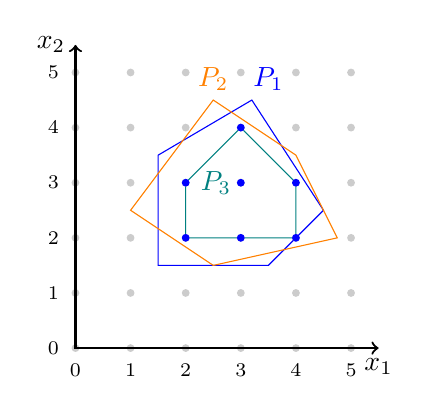
\begin{tikzpicture}[scale = 0.7,
	point/.style={circle, fill=gray!40, inner sep=1pt},
	feas point/.style={circle, fill=blue, inner sep=1pt}]
		\draw[blue] (3.2, 4.5) -- (1.5, 3.5) -- (1.5,1.5) -- (3.5, 1.5) -- (4.5, 2.5)     -- cycle;
		\draw[orange] (2.5, 1.5) -- (1, 2.5) -- (2.5,4.5) -- (4, 3.5) -- (4.75, 2) -- cycle;
		\draw[teal] (2, 2) -- (2, 3) -- (3, 4) -- (4, 3) -- (4, 2) -- cycle;  
		\foreach \x in {0,...,5}{
		  \foreach \y in {0,...,5} {
		      \node[point] (\x,\y) at (\x, \y) {};
		  }}
		\foreach \x in {0,...,5}{
		  \node[font=\scriptsize] at (\x,-0.4) {$\x$};
		}
		\foreach \y in {0,...,5}{
		  \node[font=\scriptsize] at (-0.4,\y) {$\y$};
		}                      
		\draw[thick, <->] (5.5,0) node[below]{$x_1$} -- (0,0) -- (0,5.5) node[left]{$x_2$};             
		\node[feas point] at (2,2){};
		\node[feas point] at (3,2){};
		\node[feas point] at (2,3){};
		\node[feas point] at (3,3){};
		\node[left] at (3,3){\color{teal}{$P_3$}};
		\node[above] at (2.5,4.5){\color{orange}{$P_2$}};
		\node[above] at (3.5,4.5){\color{blue}{$P_1$}};
		\node[feas point] at (3,4){};
		\node[feas point] at (4,3){};
		\node[feas point] at (4,2){};
	\end{tikzpicture}
	\caption{An illustration of three alternative formulations for $X$. Notice that $P_3$ is an ideal formulation, representing the convex hull of $X$.} \label{p1c8:fig:alternative_formulations}
\end{figure}

The formulation $P_3$ has a special feature associated with it. Notice how all extreme points of $P_3$ belong to $X$. This has an important consequence. That implies that the solution of the original integer programming problem can be obtained by solving a single LP relaxation, since the solution of both problems is the same. This is precisely what characterises an \emph{ideal} formulation, which is that leading to a minimal (i.e., only one) number of required LP relaxation solutions as solving an LP relaxation over an ideal $P$ yields a solution $x \in X$ for any cost vector $c$. This will only be the case if the formulation $P$ is the \emph{convex hull} of $X$.

This is the case because of two important properties relating the set $X$ and its convex hull $\conv(X)$. The first is that $\conv(X)$ is a polyhedral set and the second is that the extreme points of $\conv(X)$ belong to $X$. We summarise those two facts in Proposition \ref{p1c8:prop:polyhedra_convex_hull}, to which we will refer shortly. Notice that the proof for the proposition can be derived from Definition \ref{p1c2:def:convex_combination_hull} and Theorem \ref{p1c2:thm:convexity}.
  
\begin{proposition}\label{p1c8:prop:polyhedra_convex_hull}
	$\conv(X)$ is a polyhedral set and all its extreme points belong to $X$. 
\end{proposition}

%TODO: Chp7: add a proof.
 
If $P$ is such that $P = \conv (X)$, the original problem 
%
\begin{equation*}
	\mini\braces{c^\top x : x \in X},
\end{equation*}
%
can, in principle, be replaced with 
%
\begin{equation*}
	\mini\braces{ c^\top x : x \in \conv(X)},	
\end{equation*}
%
where we have that 
%
\begin{equation*}
	X = \braces{Ax \leq b, x \in \integers^n \times \reals^p} \text{ and } \conv(X) = \braces{Ax \leq b, x \in \reals_+^{n+p}}.	
\end{equation*}

Unfortunately, this is often not the case. Typically, with exception of some specific cases, a description of $\conv(X)$ is not known and deriving it algorithmically requires impractical computational requirements. However, Proposition \ref{p1c8:prop:polyhedra_convex_hull} allows us to define a structured way to compare formulations. This is summarised in Definition \ref{p1c8:def:better_formulations}.

\begin{definition} \label{p1c8:def:better_formulations}
  Given a set $X\subseteq \integers^n\times\reals^n$ and two formulations $P_1$ and $P_2$ for $X$, $P_1$ is a \emph{better formulation} than $P_2$ if $P_1 \subset P_2$. 
\end{definition}

Definition \ref{p1c8:def:better_formulations} gives us a framework to try to demonstrate that a given formulation is better than another. If we can show that $P_1 \subset P_2$, then, by definition (literally), $P_1$ is a better formulation than $P_2$. Clearly, this is not a perfect framework, since, for example, it would not be useful for comparing $P_1$ and $P_2$ in Figure \ref{p1c8:fig:alternative_formulations}, and, in fact, there is nothing that can be said a priori about the two in terms of which will render the better performance. Often, in the context of MIP, this sort of analysis can only rely on careful computational experimentation. 

A final point to make is that sometimes one must compare formulations of distinct dimensions, that is, with a different number of variables. When that is the case, one can resort to projection, as a means to compare both formulations onto the same space of variables. 

\section{Exercises}

\subsection*{Exercise 8.1: Uncapacitated lot sizing (ULS) formulations}
Consider the following formulations $P_{\text{ULS-1}}^{(x,s,y)}$ and $P_{\text{ULS-2}}^{(w,y)}$ as linear (i.e., continuous) relaxations for the ULS problem defined over $N = \{1,\dots,n\}$ periods:
\renewcommand*{\arraystretch}{1.1}
\[P_{\text{ULS-1}}^{(x,s,y)} = \left\{
  \begin{array}{llr}
  	(x,s,y): & s_{t-1} + x_t = d_t + s_t, & \forall t\in N\\
    	     & x_t  \leq M y_t, 		  & \forall t\in N\\
    	     & s_0 = 0, 			      & 			  \\
    	     & s_t \geq 0, 				  & \forall t\in N\\
    	     & x_t \geq 0, 			      & \forall t\in N\\
    	     & 0 \leq y_{t} \leq 1, 	  & \forall t\in N
  \end{array}\right\}
  \quad~\left|
  \begin{array}{rr}
  	x_t  & \text{production in period } t\\
    s_t  & \text{stock in period }      t\\
    y_t  & \text{setup in period }      t\\[5pt]
    d_t  & \text{demand in period }     t\\
    M    & \text{maximum production}\\
%         & \text{capacity}\\
         & M = \sum_{t\in N}d_t
  \end{array}\right.
\]\\[-30pt]


\[~~~P_{\text{ULS-2}}^{(w,y)} = \left\{
  \begin{array}{llr}
    (w,y): & \sum \limits_{i=1}^t w_{it} = d_t, &\forall t\in N\\
    	   & w_{it} \leq d_t y_i,  				&\forall i,t\in N : i\leq t\\
    	   & w_{it} \geq 0,        				&\forall i,t\in N : i\leq t\\
    	   & 0 \leq y_{t} \leq 1,  				&\forall t\in N 
  \end{array}\right\}
  \quad~~\left|
  \begin{array}{rr}
  	w_{it} & \text{production in period } i\\
      	   & \text{to be used in period } t\\[3pt]
       y_t & \text{setup in period } t\\
       	   & \\[7pt] 
  \end{array}\right.
\]

\vspace{5pt}

(a) Use projection to show that $P_{\text{ULS-2}}^{(w,y)}$ is stronger than $P_{\text{ULS-1}}^{(x,s,y)}$, i.e, $P_{\text{ULS-2}}^{(w,y)} \subset P_{\text{ULS-1}}^{(x,s,y)}$.

\emph{Hint:} 
First, construct an extended formulation $P_{\text{ULS-2}}^{(x,s,y,w)}$ by writing the variables $x_t$ and $s_t$ in terms of variables $w_{it}$ and add them to $P_{\text{ULS-2}}^{(w,y)}$. Then, use a projection to show that 
\begin{equation*}
\proj_{x,s,y}\,(P_{\text{ULS-2}}^{(x,s,y,w)}) \subseteq P_{\text{ULS-1}}^{(x,s,y)},
\end{equation*} 
which is equivalent to $P_{\text{ULS-2}}^{(w,y)} \subseteq P_{\text{ULS-1}}^{(x,s,y)}$. Do this by verifying that each constraint of $P_{\text{ULS-1}}^{(x,s,y)}$ is satisfied by all $(x,s,y)\in P_{\text{ULS-2}}^{(x,s,y,w)}$. Finally, show that a solution $(\bar{x},\bar{s},\bar{y})$ with $\bar{x}_t = d_t$ and \lb $\bar{y}_t = d_t/M$, for all $t \in N$, satisfies $(\bar{x},\bar{s},\bar{y}) \in P_{\text{ULS-1}}^{(x,s,y)} \setminus P_{\text{ULS-2}}^{(x,s,y,w)}$.

\vspace{5pt}

(b) The optimisation problems associated with the two ULS formulations are
\begin{align*}
	\begin{array}{lrlr}
		\text{(ULS-1)} & \mini\limits_{x,s,y} & \sum\limits_{t\in N} (f_ty_t + p_tx_t + q_ts_t)\\
		         & \st  & s_{t-1} + x_t = d_t + s_t, & \forall t\in N\\
		    	 &      & x_t  \leq M y_t, 		  & \forall t\in N\\
		    	 &      & s_0 = 0, 			      & 			  \\
		    	 &      & s_t \geq 0, 			  & \forall t\in N\\
		    	 &      & x_t \geq 0, 			  & \forall t\in N\\
		    	 &      & 0 \leq y_{t} \leq 1, 	  & \forall t\in N
	 \end{array}
	 \quad~\left|
	 \begin{array}{rr}
	  	x_t  & \text{production in period } t\\
	    s_t  & \text{stock in period }      t\\
	    y_t  & \text{setup in period }      t\\[5pt]
	    d_t  & \text{demand in period }     t\\
	    M    & \text{maximum production}\\
	 %         & \text{capacity}\\
	         & M = \sum_{t\in N}d_t
	 \end{array}\right.
\end{align*}\\[-30pt]

\begin{align*}
	\begin{array}{lrlr}
		\text{(ULS-2)} & \mini\limits_{w,y} & \multicolumn{2}{c}{\sum \limits_{t \in N} \brackets{f_ty_t + p_t\sum \limits_{i=t}^{n}w_{ti} + q_t\sum\limits_{i=1}^{t}\left(\sum \limits_{j=i}^{n}w_{ij} - d_i\right)}}\\
		               & \st                & \sum \limits_{i=1}^t w_{it} = d_t, &\forall t\in N\\              
		    	       &                    & w_{it} \leq d_t y_i,  			 &\forall i,t\in N : i\leq t\\  
		    	       &                    & w_{it} \geq 0,        			 &\forall i,t\in N : i\leq t\\  
		    	       &                    & 0 \leq y_{t} \leq 1,  			 &\forall t\in N                   
    \end{array}
    \quad~\left|
    \begin{array}{rr}
 	  	w_{it} & \text{production in period } i\\
 	      	   & \text{to be used in period } t\\%[3pt]
 	       y_t & \text{setup in period } t\\
 	       	   & %[20pt] 
    \end{array}\right.
\end{align*}\\[-20pt]

Consider a ULS problem instance over $N = \{1,\dots,6\}$ periods with demands $d = (6,7,4,6,3,8)$, set-up costs $f = (12,15,30,23,19,45)$, unit production costs $p = (3,4,3,4,4,5)$, unit storage costs \lb $q = (1,1,1,1,1,1)$, and maximum production capacity $M = \sum_{i=1}^6d_j = 34$. Solve the problems ULS-1 and ULS-2 with Julia using JuMP to verify the result of part (a) computationally.

\subsection*{Exercise 8.2: TSP formulation - MTZ}
Show that the following formulation $P_{MTZ}$ is valid for the TSP defined on a directed graph \lb $G = (N,A)$ with $N = \{1,\dots,n\}$ cities and arcs $A = \{(i,j) : i,j\in N, i\neq j\}$ between cities.
\renewcommand*{\arraystretch}{1.3}
\[P_{MTZ} = \left\{
   \begin{array}{ll}
   \displaystyle \sum_{j \in N \setminus \{i\}} x_{ij} = 1, & \forall i \in N \\
   \displaystyle \sum_{j \in N \setminus \{i\}} x_{ji} = 1, & \forall i \in N \\   
   \displaystyle u_{i} - u_{j} + (n-1) x_{ij} \leq n - 2, & \forall i,j \in N \setminus \{ 1 \} : i \neq j ~~(*)\\
    x_{ij} \in \{0,1\}, & \forall i,j \in N : i\neq j\\
  \end{array}
\right.
\]
where $x_{ij} = 1$ if city $j\in N$ is visited immediately after city $i \in N$, and $x_{ij} = 0$ otherwise. Constraints $(*)$ with the variables $u_i \in \reals$ for all $i\in N$ are called \emph{Miller-Tucker-Zemlin} (MTZ) subtour elimination constraints. 

\emph{Hint:} Formulation $P_{MTZ}$ is otherwise similar to the formulation presented, except for the constraints $(*)$ which replace either the cutset constraints
$$\sum_{i \in S}\sum_{j \in N \setminus S}x_{ij} \geq 1, \ \forall S \subset N, S \neq \emptyset,$$
or the subtour elimination constraints        
$$\sum_{i \in S}\sum_{j \in S}x_{ij} \leq |S|-1, \ \forall S \subset N, 2 \leq |S| \leq n-1,$$
which are used to prevent subtours in TSP solutions. Thus, you have to show that: 
\begin{enumerate}
\item Constraints $(*)$ prevent subtours in any solution $x\in P_{MTZ}$.
\item Every TSP solution $x$ (on the same graph $G$) satisfies the constraints $(*)$.
\end{enumerate}
You can prove 1. by contradiction. First, assume that a solution $x\in P_{MTZ}$ has a subtour with $k$ arcs $(i_1,i_2),\dots,(i_{k-1},i_k),(i_k,i_1)$ and $k$ nodes $\{i_1,\dots,i_k\} \in N\setminus\{1\}$. Then, write the constraints $(*)$ for all arcs in this subtour and try to come up with a contradiction.

You can prove 2. by finding suitable values for each $u_2,\dots,u_n$ that will satisfy the constraints $(*)$ for any TSP solution $x$. Recall that a TSP solution represents a \emph{tour} that visits each of the $N = \{1,\dots,n\}$ cities exactly once and returns to the starting city.


\subsection*{Exercise 8.3: TSP implementation}
Solve a 15 node TSP instance using the formulation $P_{MTZ}$ presented in Exercise 8.1. You can randomly generate city coordinates in x-y plane for all $N = \{1,\dots,n\}$ cities. Letting $c_{ij}$ denote the distance between cities $i$ and $j$, the problem MTZ can be formulated as
%
\begin{align*}
	(MTZ) : \mini_{x,u} & ~~\,\sum_{i\in N}\sum_{j\in N} c_{ij}x_{ij}\\
		    \st & \sum_{j \in N \setminus \{i\}} x_{ij} = 1, & \forall i \in N, \\
		        & \sum_{j \in N \setminus \{i\}} x_{ji} = 1, & \forall i \in N, \\   
		        & ~~\,u_{i} - u_{j} + (n-1) x_{ij} \leq n - 2, & \forall i,j \in N \setminus \{ 1 \} : i \neq j,\\
		        & ~~\,x_{ij} \in \{0,1\}, & \forall i,j \in N : i\neq j.
\end{align*}
%
Implement the model and solve the problem instance with Julia using JuMP.

\subsection*{Exercise 8.4: TSP formulation - tightening the MTZ formulation}
Recall the MTZ formulation for the Travelling Salesperson Problem (TSP) presented in Exercise 8.2. 

(a) Show that the inequalities \eqref{eq:31} - \eqref{eq:34} are valid for the TSP problem (i.e., they hold for any feasible solution of the TSP problem), assuming that $n > 2$:

\begin{align}
&x_{ij} + x_{ji} \leq 1, &\forall i,j \in N : i\neq j\qquad\label{eq:31}\\[5pt]
&u_i - u_j + (n-1)x_{ij} + (n-3)x_{ji} \leq n-2,   &\forall i,j \in N\setminus\{1\} : i \neq j\qquad\label{eq:32}\\[5pt]
&u_j - 1 + (n-2)x_{1j} \leq n - 1 &\forall j \in N\setminus\{1\}\qquad\\[5pt]
&1 - u_i + (n-1)x_{i1} \leq 0 &\forall i \in N\setminus\{1\}\qquad\label{eq:34}
\end{align}

\emph{Hint:} You can assume that the variables $u_2,\dots,u_n$ take unique integer values from the set $\{2,\dots,n\}$. That is, we have $u_i\in \{2,\dots,n\}$ for all $i = 2,\dots,n$ with $u_i \neq u_j$ for all $i,j\in 2,\dots,n$. This holds for any TSP solution of problem MTZ as we showed in Exercise 8.2. If we fix city 1 as the starting city, then the value of each $u_i$ represents the position of city $i$ in the TSP tour, i.e., $u_i = t$ for $t = 2,\dots,n$ if city $i\neq1$ is the $t$:th city in the tour. You have to check that each of the inequalities \eqref{eq:31} - \eqref{eq:34} hold (individually) for any arc $(i,j)\in A$ and city $i\in N$ that are part of the inequality, by checking that the following two cases are satisfied: either $x_{ij} = 0$ or $x_{ij} = 1$.


(b) Add all four sets of inequalities \eqref{eq:31} - \eqref{eq:34} to the MTZ formulation and compare the computational performance against the model with no extra inequalities.
%\emph{Hint:} The inequalities \eqref{eq:32} \emph{dominate} the original subtour elimination constraints \eqref{eq:MTZ}, so you can also try to solve the problem by commenting over the original constraints \eqref{eq:MTZ} after adding the valid inequalities \eqref{eq:32}. 


\subsection*{Exercise 8.5: Scheduling problem}
A set of $N = \{1,\dots,n\}$ jobs must be carried out on a single machine that can do only one job at a time. Each job $j\in N$ takes $p_j$ hours to complete. Given job weights $w_j$ for all $j\in N$, in what order should the jobs be carried out so as to minimise the weighted sum of their start times? Formulate this scheduling problem as a mixed integer-programming problem. 

%\emph{Hint:} Use variables $t_j \geq 0$ to represent start times of each job $j$, and variables $x_{ij} \in \{0,1\}$ with $x_{ij} = 1$ if job $i$ precedes job $j$ and $x_{ij} = 0$ otherwise.  

